\documentclass{article}
\usepackage[utf8]{inputenc}
\setlength{\parskip}{1em}
\usepackage{subcaption}


\title{Backup stuff}
\author{Jonathan S. Abrahams }
\date{October 2019}

\usepackage{natbib}
\usepackage{graphicx}

\begin{document}

\maketitle
 This analysis was expanded in order to determine its use in associating duplication genotypes to phenotypes when background noise is present. In parralel with the first experiment the aim was to establish a genotype-phenotype connection between the duplications in network 1 and the `perfect phenotype',however, in this experiment, the full complement of estimated duplications/deletions was used as input. This provided a more realistic scenario with confounding mutations potentially present such as duplications at other loci and lineage associated deletions. The full dataset of duplications and deletions was inputted to pySEER with deletions and duplications set to 1 and all genes at single copy set to 0. 
 
 Rerunning the analysis with all duplications and deletions as input resulted in the genes in the duplication,previously highly significant, failing statistical tests. The data showed a large discrepancy between the lineage unadjusted and lineage adjusted p values and came with warnings of low statistical power. This therefore meant that even given the `perfect' phenotype, statistical power was not achieved to associate a genotype with a phenotype using this method. 
 
 It was possible that the highly abbreviated phylogenetic tree used to inform pySEER,comparing only 10000 kmers of each sample, may have underestimated the fine scale structure of B.pertussis phylogenies. The analysis was therefore rerun with a phylogenetic tree based on core genome SNPs which had much higher resolution. This minor changes to the methodology,however, did not change the results signficantly.Even increading the number of principal compnenets usedi n the analysis, potentially introducing false positives, did not increase the statistical power.
 
 
 %this just isnt true. This method could be great! We need to test this method with SNPs and CNVs tested alongside each other But.. hasnt this already been tested? the phylogenetic tree?
 It was therefore clear that it was impossible to use the previously generated data, a matrix of copy number estimates for each gene in each strain, to associate genotpyes with phenotyes. Other strategies were therefore investigated to undertake GWAS which not only gave significant results, but also provided a more accurate picture of the variations in the genome.
\subsection{K-mer based approach as a genotype for GWAS}
%Rewrite this to better refelct new results in previous section
Acknowledging the co-existence of all mutation types is imperative in understanding the trajectory evolution is undergoing as neutral mutations can often 'hitch-hike' on mutations which are under positive selection. Therefore analysing a genotype-phenotype link one mutation type at a time may give erroneous results. Our initial analysis of a presence/absence matrix of duplications,whilst functional in a test scenario, would be therefore flawed for use in practise. We therefore sought a rigorous method to provide a holistic genotype, of which all known mutations were inputted, for GWAS in order for a robust genotype-phenotype link to be hypothesised. 

Whilst using K-mers is the most ubiquitous strategy to define a genotype,this strategy does however poses a variety of problems for the analysis of SVs in bacteria. 

%How kmers work and why they are useful
\subsubsection{K-mer based problems}

The strength and ubiquitous use of K-mers in bioinformatics (refs) stems from the ease K-mers bring to the challenging task of comparing two or more sequences. A K-mer is considered a match to a target sequence only if it is an exact match, therefore avoiding the array of complications stemming from approximate matching of larger sequences. The sensitivity and specificity of this 'exact match' property of K-mers is dependent on the length of the kmer and of the variability of the target sequence in addition to other influences. For example, longer K-kmers are more specific bus less sensitive. 


%Point 1: Structural variations
For most GWAS applications, the K-mer length is not a critical variable to the analysis as increasing or decreasing the kmer size produces the expected linear effect on sensitivity and specificity. However, the length of the repeats involved in recombination-mediated SVs often exceeds the length of K-mers used in GWAS- such mutations are rendered `invisible' to K-mer based GWAS analysis. There are a variety of different solutions to this problem, each with advantages and disadvantages.

A seemingly clear solution to study SVs with K-mers would be to increase the K-mer length to exceed the length of the repeats of interest which often exceed 1kb in length. The length of K-mers is a balance between sensitivity and specificity,however, and therefore  long (100bp+) K-mers may lead to extremely high specificity (Figure \ref{fig:Sens_spec}). In the highly clonal bacterium B. pertussis, which most often contain 20-300 SNVs in the 4.1Mb genome, very long K-mers were still informative, but such K-mers in other species would be too specific.

\subsubsection{Kmer length }

To investigate how kmer length affects sensitivity and specificity in BP, a trial experiment was undertaken. Samples of 1000 K-mers were taken for each of the ~500 closed BP genomes at kmer lengths of 21-1001. Using this data phylogenetic trees can be made. Overly sensitive K-mers will produce a more 'star-like' tree where each strain appears more unrelated to another whilst overly specific kmers will produce an overly flat tree, overestimating the relationships between isolates. Therefore if trees made using long kmers were considerably more 'star-like' then it was evident that such kmers were too long to be of any use in B.pertussis.



%Perhaps here, include a graph with real data showing this effect: how does kmer length influence interspecies and intra species resolution of isolates?. However, alot of effort for a mionor point.



Another strategy is to exclude repeat regions, meaning the `pre-repeat' and `post-repeat' sequence are adjacent and thus novel junctions can be captured by regular length K-mers. However, there is evidence that specific IS alleles have different regulatory effects on adjacent genes and thus the exclusion of these sequences may mask specific repeat allele associations with genomic loci. Both strategies were investigated here in order to elucidate the most effective strategy with reference to B.pertussis and more generically, to the bacterial kingdom as a whole.

\subsubsection{K-mer abundance is a reliable proxy for copy number but pySEER cant analyse it}

Using K-mer abundunce as a marker to establish a genotype-phenotype link was investigated.

A small number of highly related isolates were used, stemming form the Weigand et al study: one strain with a duplication and two strains without the duplication. All strains had been used to generate vaccines against BP in India.

It was first investigated if the strain with a duplication had a higher kmer abundunce in the expected region compared to the two control strains without the duplication. This required generating kmers with FSM-lite for the three strains and mapping the kmers to a reference genome. The reference genome used was the genome with the duplication. All-kmers were used including those which mapped to all genomes and those that only mapped to one genome- these are often excluded but were included here for completeness.

Which part of the genome contained kmers that were present more in the duplication genome than in the control genome was investigated. Our results indicated that these kmers occurred much more frequently in the duplication region compared to the rest of the genome (Fig. \ref{fig:Kmer_abund_is_dece}), even when only the primary alignment was used (Fig. \ref{fig:Kmer_abund_supp_off}). There were many kmers outside of the duplication that were present more often in the duplication genome compared to the control genome, however. To remedy this, only kmers that occur a single time in the control genomes and two times in the duplication genome were used.

%Probably should merge these graphs. The second one may not be appropriate at all, too much info. In fact. maybe just skip this bit and go straight to the graph with unique kmers? Or perhaps a density plot to combine all three.
 \begin{figure}[h!]
\centering
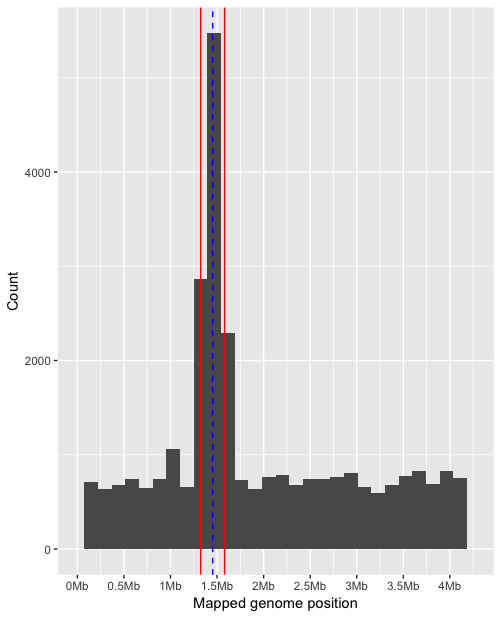
\includegraphics[width=\textwidth]{Chapter_3/Kmer count dupe signal.png}
\caption{Kmers that were more abundant in the genome with the duplication were mapped to the reference genome (X) and a histogram produced. It was clear that there were a high count (Y) of these kmers in the region containing the two copies which is bounded by the red lines. The blue line indicates the junction between the duplicate regions.}
\label{fig:Kmer_abund_is_dece}
\end{figure}

 \begin{figure}[h!]
\centering

\includegraphics[scale=0.6]{universe.jpg}
\caption{Same as above graph but we switch off supplementary alignments.}
\label{fig:Kmer_abund_supp_off}
\end{figure}

\begin{figure}[h!]
\centering
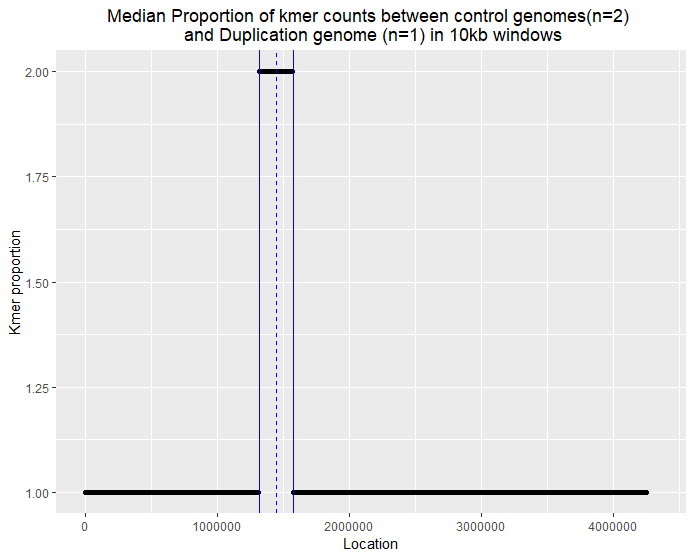
\includegraphics[scale=0.6]{Kmer_dupe.png}
\caption{We can identify the boundry of a dupe using kmers}
\label{fig:kmer_dupe1}
\end{figure}

%But can pyseer analyse this data?

%The initial go at this didnt pick out any kmers at all that were significant.

\subsubsection{Ultra-long K-mers overcome the problem}

%a subsample of ultra long kemrs at 1300bp, longer than a single IS, were significant for the IS boundary.
%This is of limited use, what if there was variation around this? need to make kmers between 20-1300 and also use a more representative sample to get the chi2 test to work.

In order to test the efficacy of long kmers, a simple trial was conducted. Two genomes 
Kmers ranging from 21-1300 in length were tested for a trial dataset

%Ultra long kmers overcome the problem that kmers are smaller than repeats, however this may not be so applicable to more diverse bacterium outside of B.pertussis.

\subsubsection{Excluding repeat regions overcome the problem}

%Excluding repeat regions was the best solution. However rearangements.





\begin{figure}[h!]
\centering

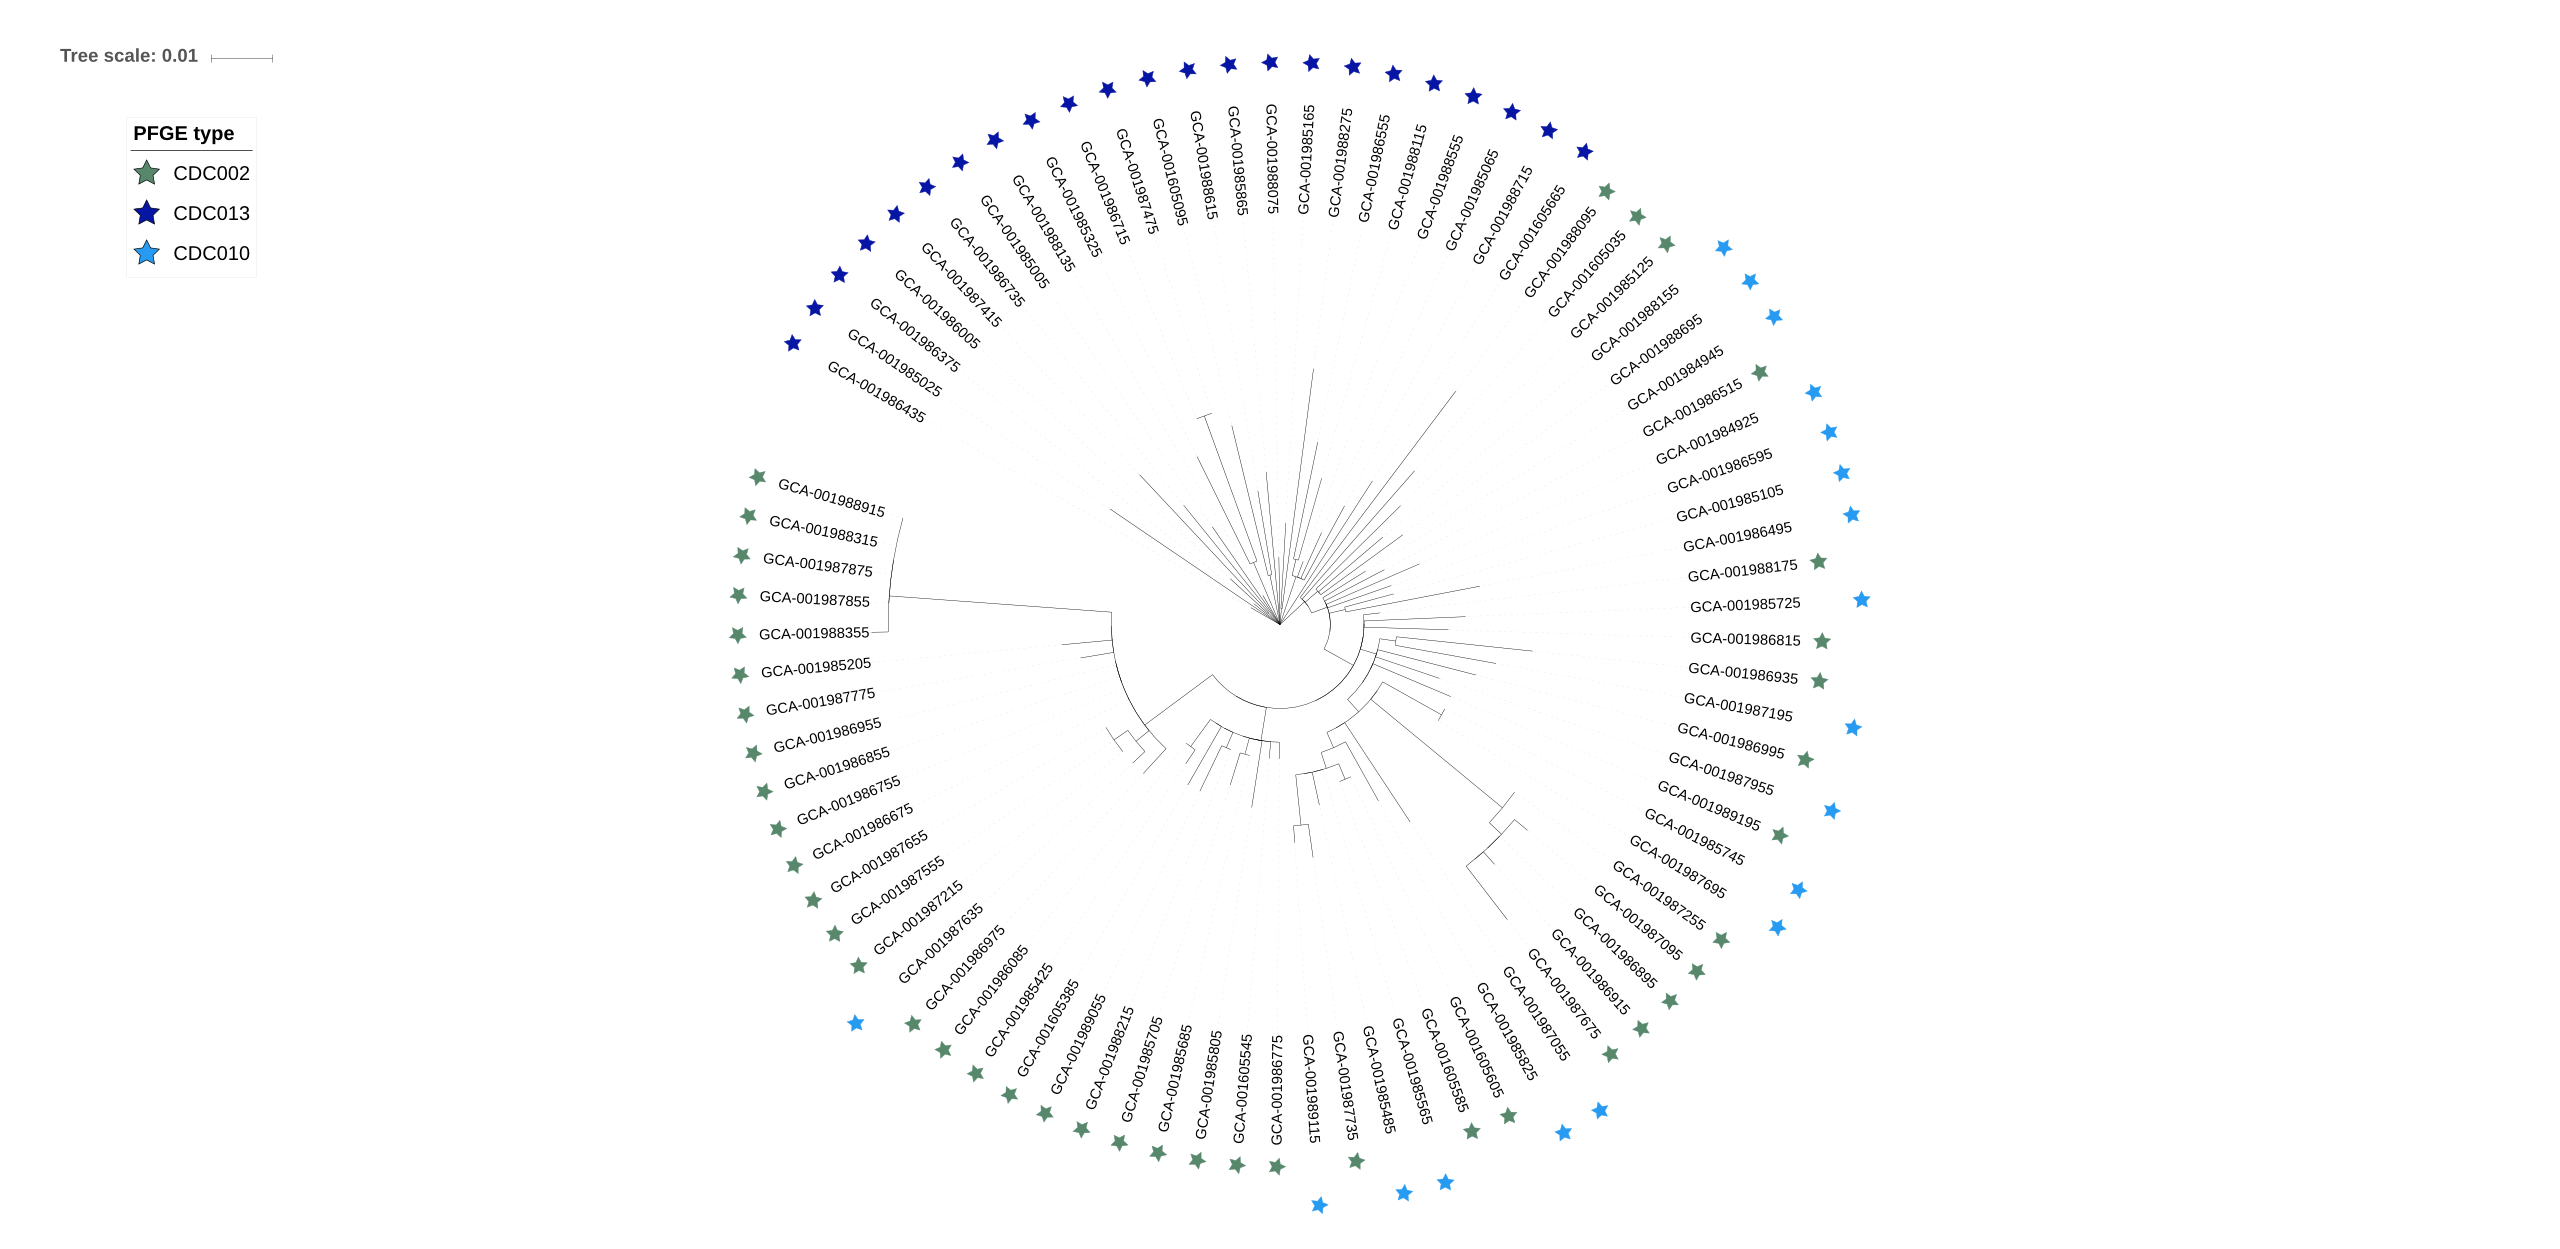
\includegraphics[width=\textwidth{}]{PFGE_tree.png}
\caption{PFGE types are homoplasic}
\label{fig:PFGE_tree}
\end{figure}


%This figure will be a manhatten plot of this

\subsection{Establishing a link between SV and phenotype in TB}
Pre-amble about why TB.
\subsubsection{}


%\bibliographystyle{plain}
%\bibliography{references}
\end{document}
